In this section we describe a few additional options and functions that the pipeline has to offer.

\subsection{Walltime and RAM Approximation and Addition}
Currently, walltime and RAM are approximated using the needed time and RAM from previously benchmarked datasets. For each step it calculates $\frac{walltime}{numberOfCells}$ and $\frac{RAM}{numberOfCells}$ for each dataset and uses the greatest gradient as factor. This gradient is then multiplied by the number of the cells of the dataset you wish to process as an approximation. 

However, if the approximation is not enough for the HHU HPC you can increase it by adding a few GB RAM of a bit walltime in seconds into the snakemakeScripts/Pipelineoptions.py "addRAM" and "addTime" dictionaries for the steps that need it respectively. You can also add them at the very beginning if you do not trust the approximation.

\subsection{Benchmarking}
If you want to do some benchmarking to add to the approximation then you first need to remove the comments marks for the benchmarking in the Snakefile and increase execTimes to the number of times each step should be executed for each benchmark.

\subsection{Seurat and Snakemake Parallelization}
Seurat offers parallelization of certain functions by using the Future package. In snakemakeScripts/PipelineOptions.py you can increase the number of cores for certain steps to decrease the walltime. All steps that \textbf{do not} have the multicore functions are marked with an X.

The pipeline itself also offers some parallelization functions. In the beginning the dataset is split into its individual sample (e.g. split into each patient). These samples can be processed simultaneously and independently from each other. If you run the pipeline on the HHU HPC you do not need to do any extra steps for this parallelization.

If you do not run the pipeline on the HHU HPC, but via the snakemake command, you need to set X in the snakemake option "--cores X" to the maximum number of cores you want to use.

\begin{figure}[h!]
	%\includesvg[width=\textwidth]{figures/pipelineRun.pdf}
	\centering
	\makebox[\textwidth][c]{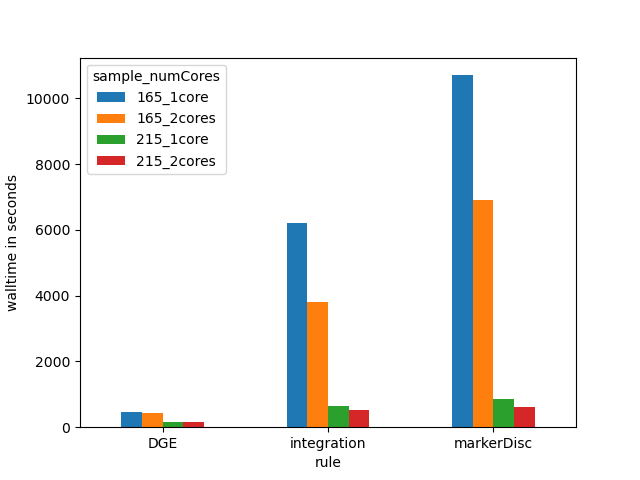
\includegraphics[width=1\textwidth]{figures/paraFutureBars.png}}
	\caption{Walltime reduction through parallelization with Seurat and Future.}
	\label{fig:parallelBars}
\end{figure}

\subsection{Conda Environments}
You can create your own folder with your own conda\_envs.yaml in the envs/ folder and change the environments in snakemakeScripts/PipelineOptions.py in the else case of the "setCondaEnv" function if you do not run the pipeline on the HHU HPC.
